\subsection{Controller Subsystem}
\label{sec:controller_subsystem}
\begin{figure}[H]
    \label{mcu_block_diagram}
    \caption{MCU block diagram}
    \centering
    % Need to update block diagram
    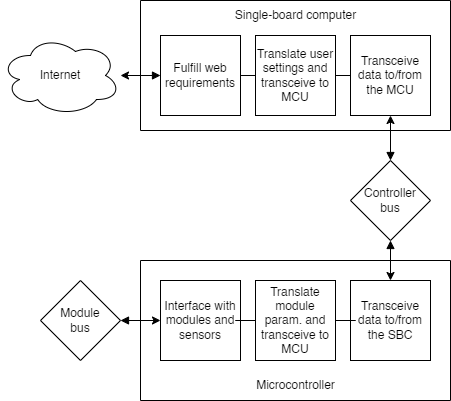
\includegraphics[width=0.75\textwidth]{images/mcu_block_diagram.png}
\end{figure}
% I need to write 11 pages lmfao
\begin{flushleft}
    % Why the MCU connects to the internet
    In order for our system to be as self-sufficient and power efficient as
    possible from an end-user perspective, it was determined that our system
    would require an internet connection to offload remote command-and-control
    to an Amazon Web Services EC2 instance (hence referred to as "AWS" and detailed in
    \autoref{sec:web_subsystem}). To make the process of operating our product 
    as hands-off as possible to end-users, the microcontroller will connect to
    the user's home WiFi network for access to AWS. Bluetooth, Zigbee, Thread,
    and other short-range 2.4 GHz communication protocols were disfavored over
    WiFi, as we predict most users will not have a device to dedicate to
    connecting our product via such protocols. Long range (LoRa) protocols were
    deemed unncessary, as the intended placement of our product is outside, 
    near or next to the user's home. We do not expect our product to produce
    or receive large amounts of data, so the decreased bandwidth of a
    WiFi-enabled product being beyond the outdoor walls of a building
    is not a significant drawback to our application. A wired connection
    (802.3/Ethernet) was deemed too invasive to the end-user. It is expected
    that most, if not all, end-users have a wireless access point and internet
    access. Thus, connection via the 802.11/WiFi standard was a natural choice
    for our use case.
\end{flushleft}
\begin{flushleft}
    % How the MCU connects to the internet (local network, LAN -> NAT -> WAN,
    % TCP stack)
    The Texas Instruments CC3220-series of microcontrollers are WiFi-enabled
    chips with an ARM Cortex-M4 central processor and a WiFi network processor,
    along with many useful peripherals and power management modules. The WiFi
    network processor supports the following standards/features useful to our
    development:
    \begin{itemize}
        \item WiFi standards: 802.11b/g/n
        \item WiFi security: WEP, WPA/WPA2 PSK, WPA2 enterprise, WPA3 personal,
        WPA3 enterprise
        \item WiFi provisioning: SmartConfig, WPS2
        \item IP protocols: IPv4, IPv6
        \item IP addressing: static IP, DHCPv4, DHCPv6
        \item Transport: UDP, TCP, RAW
        \item Host interface: UART, SPI
        \item Built-in transceiver and 2.4 GHz antenna
    \end{itemize}
    Our microcontroller will 
    % WHAT KIND OF INTERFACE????
    % option a) web interface for user to long in to WLAN
    % option b) WPS button
    % don't forget IP addressing (most likely DHCP)
\end{flushleft}
\begin{flushleft}
    % TCP sockets
\end{flushleft}
\begin{flushleft}
    % Parameters for connection and how often it tries
    Once the MCU has established a connection to the internet and the AWS
    instance, it attempts to send current system settings and telemetry, as
    well as sensor readings to AWS. The microcontroller does this at least
    once every 15 minutes. Sending and receiving may occur more often if
    commanded to by AWS. Because TCP is being used to connect AWS and the
    microcontroller, any manual retries on a failed send or receive most
    likely will be futile. Therefore, any sort of link error handling will
    be performed by the link and not the microcontroller program.
\end{flushleft}
\begin{flushleft}
    % Any over-the-air updates?
    At this time, our team does not intend to provide a method for over-the-air
    updates (OTA), however, this is a provision that may be developed in the
    future.
\end{flushleft}
\begin{flushleft}
    % MCU receives commands, decodes commands
    The MCU will receive commands and data from AWS in the following form:
    \begin{center}
        \texttt{t x c y}
    \end{center}
    where \texttt{t} (character) marks the beginning of the command string,
    \texttt{x} (unsigned integer) indicates how many seconds to wait before
    executing command \texttt{c} (character) with parameter \texttt{y}
    (ambiguous). The following characters occupy the spot of \texttt{c}, and
    translate to the following commands:
    \begin{center}
        \texttt{w y}: water, \texttt{y} is boolean \\
        \texttt{a y}: solar $\theta$, \texttt{y} is double \\
        \texttt{b y}: solar $\phi$, \texttt{y} is double \\
        \texttt{l y}: low power, \texttt{y} is unsigned int for flags \\
        \texttt{s y}: send data, \texttt{y} is unsigned int for flags
    \end{center}
    For example, if AWS instructs the MCU to turn on the water source in 3
    minutes, it would send the command \texttt{t 180 w 1}. If AWS would like
    the MCU to change the $\theta$ of the solar panels to 45$\degree$
    immediately, it would send \texttt{t 0 a 45.0}. It is important to note
    that the values of \texttt{x} and \texttt{y} are not strings (e.g.
    45$\degree$ will not be sent as \texttt{"45.0"}), but the actual encoding
    of 45$\degree$ as a double-precision float. This is to maintain a
    consistent command string size amongst all transmissions.
    \begin{figure}[H]
        \label{command_bitwise}
        \caption{Bitwise representation of command}
        \centering
        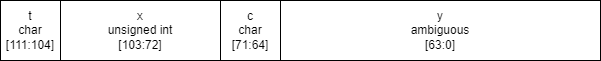
\includegraphics[width=0.75\textwidth]{images/command_encoding.png}
    \end{figure}
\end{flushleft}
\begin{flushleft}
    % Will program in C++. Any libraries, multithreading?
    It should be expected that all headers from the C++ standard library (as
    defined in C++23) will be used, along with the following nonstandard
    libraries: \texttt{TBD}. Additionally, it is expected that the MCU program
    will run on a single thread.
\end{flushleft}
\begin{flushleft}
    % Classes and class diagram
    There will be a few classes defined in the MCU's programming:
    \begin{center}
        \texttt{Class FromWeb \{}  \\
        \texttt{uint32\_t time\_until\_exec;} \\
        \texttt{uint32\_t time\_until\_exec;} \\
        \texttt{uint32\_t time\_until\_exec;} \\
        \texttt{uint32\_t time\_until\_exec;} \\
    \end{center}


    TBD, add UML class diagrams.
    % Structs -> classes
    % Classes:
    %  Water
    %  Solar
    %  Battery/charge controller
    %  AWS/socket
    %  Telemetry (own system)
\end{flushleft}
\begin{flushleft}
    % Send to AWS, format and types of commands
\end{flushleft}
\begin{flushleft}
    % Global vars
\end{flushleft}
\begin{flushleft}
    % Functions
\end{flushleft}
\begin{flushleft}
    % Interrupts and ISRs
\end{flushleft}
\begin{flushleft}
    % How the MCU gets data from sensors (ADC)
\end{flushleft}
\begin{flushleft}
    % How MCU sends data to servos
\end{flushleft}
\begin{flushleft}
    % What sort of telemetry we'll have
\end{flushleft}
\begin{flushleft}
    % What kind of development model?
    % Probably agile
\end{flushleft}